\documentclass[a4paper, czech]{article}

\usepackage[czech]{babel}
\usepackage{indentfirst}
\usepackage{graphicx}
\usepackage{float}
\usepackage[margin=1.5cm]{geometry}
\usepackage{booktabs}
\usepackage{amsmath}
\usepackage[table]{xcolor}
\usepackage{multirow}
\usepackage{tabularray}
\usepackage{bold-extra}

\begin{document}
\begin{table}[H]
    \centering
    \begin{tblr}{
        cell{1}{1} = {c = 2, r = 4}{c}, % Logo
        cell{1}{4} = {c = 3}{c}, % Předmět
        cell{2}{4} = {c = 3}{c}, % Jméno
        cell{3}{4} = {}{c}, % Ročník
        cell{3}{6} = {}{c}, % Studijní skupina
        cell{4}{4} = {}{c}, % Spolupracoval
        cell{4}{6} = {}{c}, % Mereno dne
        cell{5}{1} = {c = 2}{55mm}, % Kontroloval
        cell{5}{3} = {c = 2}{55mm}, % Hodnoceni
        cell{5}{5} = {c = 2}{55mm}, % Dne
        cell{6}{2} = {c = 5}{}, % Nazev ulohy
        cell{7}{1} = {}{c}, % Číslo úlohy
        cell{7}{2} = {c = 5}{c}, % Název úlohy
        vline{1,2,7} = {1.2pt},
        vline{3,5},
        hline{1,5,6,8} = {1.2pt},
        hline{2,3,4}
        }
        
\includegraphics{logo_fekt.png} & & \textsuperscript{Předmět} & \large \textbf{Měření v audiotechnice} \\
             & & \textsuperscript{Jméno} & \large \textbf{Karolína Šebestová} \\
             & & \textsuperscript{Ročník} & \large \textbf{3.} & \textsuperscript{Studijní skupina} & \large \textbf{St 14:00} \\
             & & \textsuperscript{Spolupracoval} & \large \textbf{Filip Kokavec} & \textsuperscript{Měřeno dne} & \large \textbf{16.10.2024} \\
        \textsuperscript{Kontroloval} & & \textsuperscript{Hodnocení} & & \textsuperscript{Dne} \\
        \textsuperscript{Číslo úlohy} & \textsuperscript{Název úlohy} \\
        \Large \textbf{3B} & \Large \textsc{\textbf{Automatizované měření impedance reproduktoru}} \\
    \end{tblr}
\end{table}

\section{Zadání}

\begin{itemize}
    \item Seznamte se s měřením impedance metodou tří voltmetrů a Ohmovou metodou.
    \item Pomocí generátoru, osciloskopu a počítače realizujte automatizované měření kmitočtové charakteristiky impedance reproduktoru v audio kmitočtovém spektru.
    \item Z kmitočtové charakteristiky impedance určete stejnosměrný odpor, jmenovitou impedanci a rezonanční kmitočty a diskutujte vliv bassreflexového nátrubku na tyto charakteristické veličiny.
\end{itemize}

\section{Teoretický úvod}

Definice impedance dle Ohmova zákonu (poměr fázoru napětí a fázoru proudu):

\begin{equation*}
    Z = \frac{U}{I}
\end{equation*}

Jedná se o komplexní veličinu.

Jakožto prevenci proti zkratování impedance přes zemnící póly kanálů osciloskopu je možné využít diferenciálních metod měření:

\begin{itemize}
    \item \textbf{Aktivní diferenciální napěťová sonda}
    
    Umožňuje měřit napětí bez uzemnění jednoho z měřících uzlů v obvodu.
    Využívá pouze jednoho kanálu na osciloskopu.
    Vyžaduje externí napájení.
    \item \textbf{Diferenciální měření dvěma kanály osciloskopu}
    
    Využívá dvou kanálů na osciloskopu.
    Na měřící uzly jsou ppřipojené kladné póly kanálů.
    Na osciloskopu zobrazíme rozdíl mezi kanály A a B.
\end{itemize}

\textbf{Ohmova metoda:} je nutné znát napĚtí i proud na měřeném vzorku.

\textbf{Metoda tří voltmetrů:} Je nutné znát napětí zdroje na měřeném vzorku a na sériovém rezistoru.

\textbf{Impedance reproduktoru:}

\begin{itemize}
    \item Jmenovitá impedance - nejnižší hodnota impedance v pracovním kmitočtovém pásmu.
    \item Stejnosměrný odpor - na počátku kmitočtové charakteristiky impedance.
    \item Kmitočtová charakteristika impedance - nelineární, můžeme určit rezonanční kmitočty reproduktoru z lokálních maxim.
\end{itemize}

\begin{figure}[H]
    \centering
    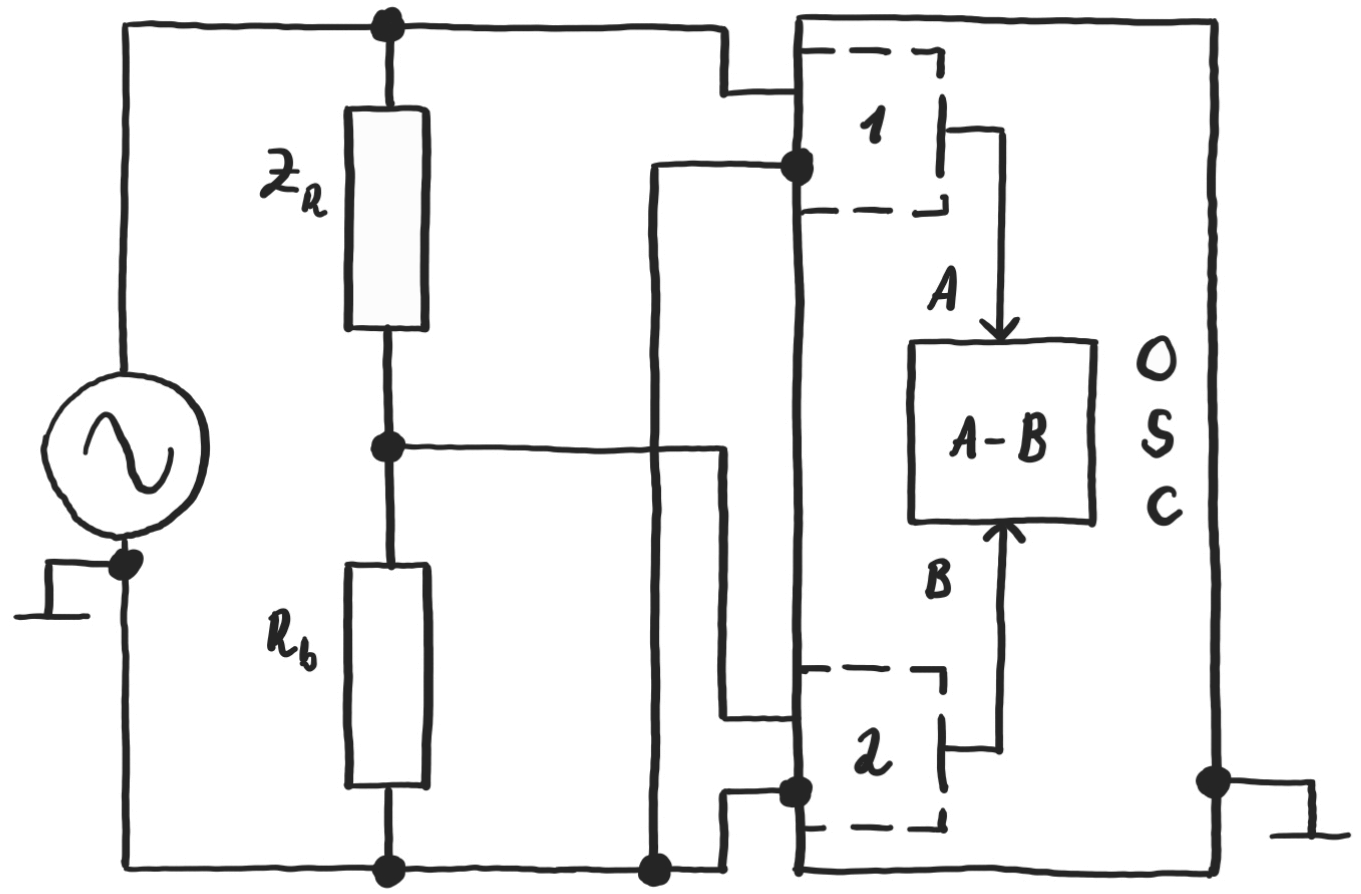
\includegraphics[width = 0.5\textwidth]{schema3b.png}
\end{figure}

\section{Výsledky měření}
 
\subsection{Tabulky}

\subsection{Grafy}

\subsection{Příklady výpočtu}

\section{Seznam použitých přístrojů}

\section{Závěr}

\end{document}